% mainfile: ../../../../master.tex
\subsection{DNA quantification with Qubit\texttrademark~ DNA BR Assay Kit}
% The part of the label after the colon must match the file name. Otherwise,
% conditional compilation based on task labels does NOT work.
\label{task:20180208_cj1}
\tags{lab,dna,rna,qnt}
\authors{cj}
%\files{}
%\persons{}

\begin{figure}[H] % position of the figure 
    \centering
    \caption{Illustration for the QubitTM DNA BR assay to quantify the DNA extracted with the AllPrep DNA/RNA Mini Kit}
    \label{fig:20180208_Qubit_dsDNA_BR}
    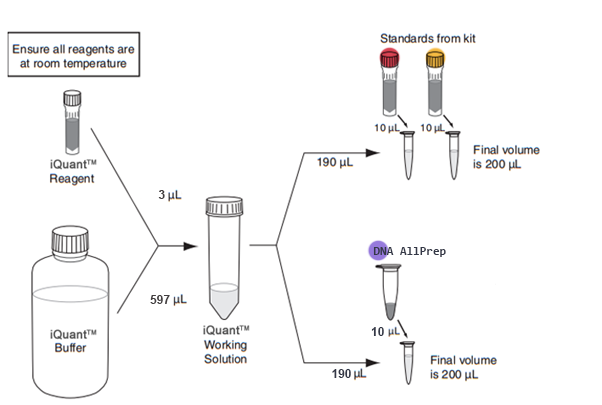
\includegraphics[width=0.7\textwidth]{graphics/schemas/20180208_Qubit_dsDNA_BR.png}
\end{figure}

\begin{table}[H]
\caption{Total cDNA quantities in samples measured with Qubit\texttrademark ~ssDNA Assay Kit}
\label{tab:20180208_dna_allprep_qnt}
\centering
\begin{tabular}{l r r r r}
\toprule
Sample ID & \textmu g/mL & $V_f$ (mL) & m (\textmu g) & m (ng) \\ \midrule
\texttt{DNA\_AllPrep} & 2.44 & 0.088 & 0.214 & 214.72 \\
\bottomrule
\end{tabular}
\end{table}

The concentration measured with the Qubit\texttrademark~ allows me to calculate the total amount of DNA obtained which is 214.72 ng of DNA. This is not bad and it should enough for an amplification by \gls{pcr}. But it is not enough for metagenomics HiSeq sequencing because the TruSeq\texttrademark~ DNA PCR-Free library preparation kit requires 1~\textmu g of DNA. 